\begin{figure}[t]
\centering
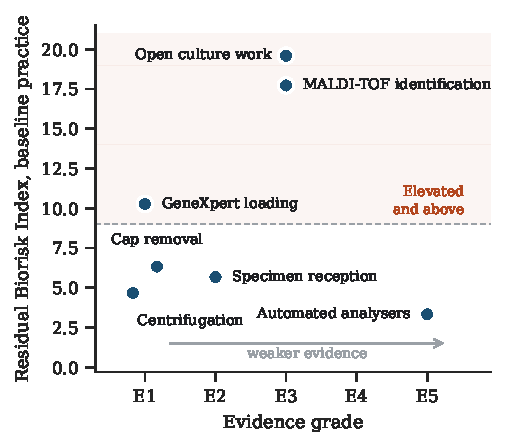
\includegraphics[width=\columnwidth]{figures/fig1_inversion.pdf}
\caption{Residual biorisk under baseline practice against the strength of the evidence
base, each point one bench step at its primary agent profile. The relationship is
negative: the two steps carrying the highest residual biorisk rest on incident evidence
with no aerosol measurement, while the lowest-scoring pre-analytical steps have been
measured directly. The highest-throughput step in the laboratory, automated analyser
operation, carries no located evidence of any kind.}
\label{fig:inversion}
\end{figure}

\begin{figure}[t]
\centering
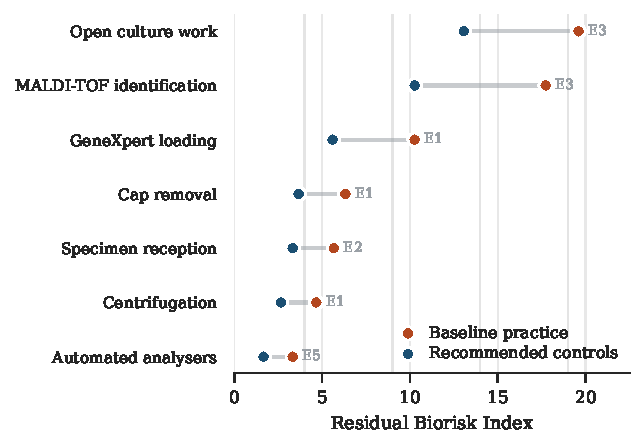
\includegraphics[width=\columnwidth]{figures/fig2_control_effect.pdf}
\caption{Movement from baseline practice to the recommended control set, each step at its
primary agent profile, ordered by baseline score. Letters give the evidence grade. The
largest reductions occur where baseline control reliability is weakest and the consequence
profile most severe, and are driven principally by moving open manipulation into a
certified Class~II biological safety cabinet. Neither of the two highest steps reaches the
Low band even with the full recommended set applied.}
\label{fig:controls}
\end{figure}

\begin{figure*}[t]
\centering
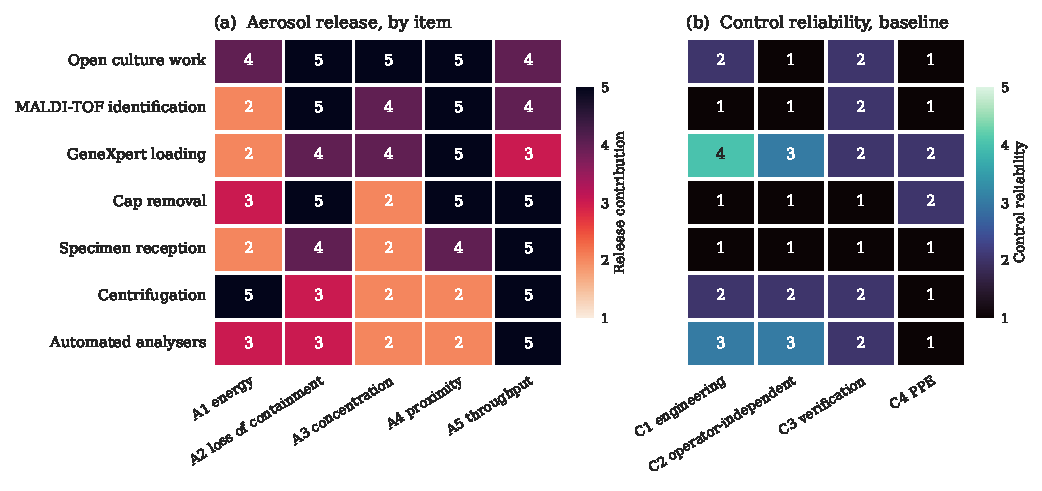
\includegraphics[width=\textwidth]{figures/fig3_item_heatmap.pdf}
\caption{Item-level decomposition, steps ordered by residual biorisk under baseline
practice. Panel (a) shows the five aerosol release items; A2 is displayed reverse-coded,
so a higher value means less containment and therefore more release. Panel (b) shows the
four control reliability items under baseline practice, with rows in the same order. Open
culture work reaches its position through a uniformly high release profile, whereas
MALDI-TOF target preparation scores low on energy and reaches a comparable position
through loss of containment, concentration and breathing-zone proximity under the most
severe consequence profile. Centrifugation shows the opposite structure: the highest
energy score in the reference, with containment, concentration and proximity all low.}
\label{fig:items}
\end{figure*}

\begin{figure*}[t]
\centering
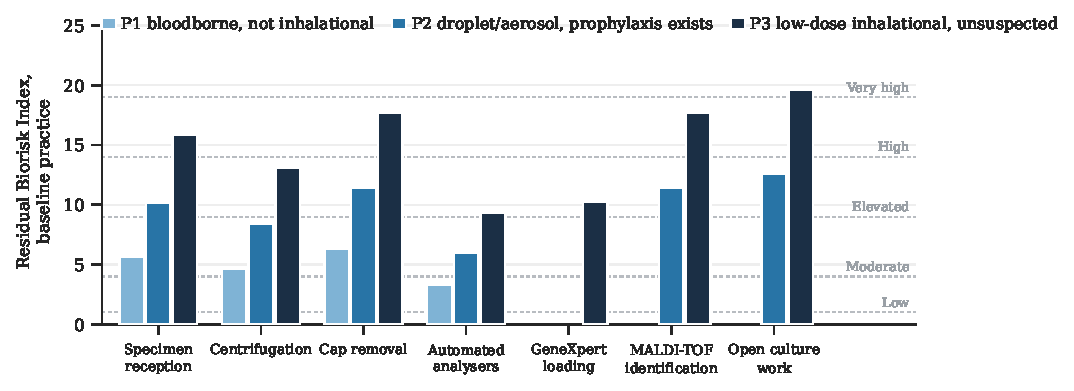
\includegraphics[width=\textwidth]{figures/fig4_profile_sensitivity.pdf}
\caption{Residual biorisk under baseline practice for every step and every applicable
agent profile. Cartridge loading is reported under P3 only, since the step exists because
a low-dose inhalational agent is suspected. The spread within a step is wide: specimen
reception ranges from 5.67 under P1 to 15.87 under P3, more than two bands apart, from
identical release and control scores. The profile assumption is therefore the single
largest determinant of where a step lands, which is why three profiles are reported rather
than one being assumed.}
\label{fig:profiles}
\end{figure*}
